\documentclass[10pt,journal,compsoc]{IEEEtran}
\usepackage[ruled,vlined]{algorithm2e}
\usepackage{multirow}
\usepackage{amsfonts}
\usepackage[cmex10]{amsmath}
% \usepackage[nocompress]{cite}
\usepackage[tight,normalsize,sf,SF]{subfigure}
\usepackage{graphicx}
\usepackage{hyperref}


\begin{document}
%opening
\title{Market-Based Multi-Agent Systems as a Self-Adaptation Mechanism in the Cloud}
\author{Vivek Nallur, Rami Bahsoon}

\IEEEcompsoctitleabstractindextext{%
\begin{abstract}
Cloud computing, with its promise of (almost) unlimited computation, storage and bandwidth, is increasingly becoming the infrastructure of choice for many organizations. As cloud offerings mature, service-based applications need to dynamically recompose themselves, to self-adapt to changing QoS requirements. In this paper, we present a decentralized mechanism for such self-adaptation, using market-based heuristics. We use a continuous double-auction  to allow applications to decide which services to choose, amongst the many on offer. We view an application as a multi-agent system, and the cloud as a marketplace where many such applications self-adapt. We show through a simulation study that our mechanism is effective, for the individual application as well as from the collective perspective of all applications adapting at the same time. We show that our mechanism is highly scalable and robust in the presence of skewed distributions of QoS demand by service consumers and supply by service providers. 
\end{abstract}

\begin{keywords}
Self-Adaptation, Market-Based, Multi-Agent Systems    
\end{keywords}
}

\maketitle

\section{Introduction}
Self-adaptation, as a concept, has been around for many years, in several domains like biology, chemistry, logistics, economics etc. Self-adaptivity in computer-based systems is relatively newer. Some of the first references to self-adaptive software systems are from \cite{Oreizy1998Architecture-based}, \cite{Laddaga1999Guest}, \cite{Kokar1999Control} and \cite{Kephart2003Vision} (where they are referred to, as autonomic systems). By self-adaptivity in software systems, we mean software that monitors itself and the operating environment, and takes appropriate actions when circumstances change. In web-applications, service-oriented architecture has often been used as a mechanism for achieving self-adaptivity\cite{DiNitto2008journey}. Web-services allow for dynamic composition, which enables applications to switch services, without going offline. A common instance of using web-services dynamically, is applications living on the cloud, asking for computing power and bandwidth to be scaled up or down, depending on demand. However, one of the cloud's major selling points, \textit{operational flexibility} is of little use, if applications (or organizations) have to indicate at sign-up time, the kind of services that they intend to use. On Amazon, for instance, a customer specifies during sign up whether she wants a Hi-CPU instance or a Standard On-Demand instance or a Hi-Memory instance. This assumes that an application is able to forecast its demand for computing and storage resources accurately. However, this inability to forecast is precisely what the cloud claims to address through elasticity in computing power. This is not to say that there are no flexible, demand-based pricing schemes available. Amazon's \textit{Spot Instances} \cite{Amazon2010SpotInstance} is an example of how cloud providers are trying to flexibly price their services, in response to fluctuating demand over time. Applications that can adapt to fluctuating prices will be able to ensure a better return on investment. In the future, we surmise that service-pricing will depend not only on demand but also on additional attributes like performance, availability, reliability, etc.
\\ 
Current implementations of public clouds mainly focus on providing easily scaled-up and scaled-down computing power and storage. We envisage a more sophisticated scenario, where federated clouds with different specialized services collaborate. These collaborations can then be leveraged by an enterprise to construct an application, that can be self-adaptive by changing the specific web-service it utilizes. The notion of utilizing collaborative services to satisfy a business need, is not new in itself. The recognition of Agile Service Networks (ASN) that spring up in modern business practices, is testament to this. 
\begin{quote}
An Agile Service Network (ASN) comprises large numbers of long-running, highly dynamic complex end-to-end service interactions reflecting asynchronous message flows that typically transcend several organizations and span geographical locations. 
\end{quote}
As ASNs mature and dynamic composition becomes the norm, we posit that applications that're composed of other applications will routinely adapt to changing QoS requirements. In this paper, we propose a decentralized mechanism to address the problem.  
\subsection{Problem Statement}
Composite web-services are services that are composed of other web-services. Several web-applications are made by composing web-services together. The effective QoS provided by such an application is a function of the QoS provided by the individual web-services. Hence, if the application wishes to exhibit a different level of QoS, it can do so by changing its constituent web-services. However this is not an easy task. Identifying the optimal web-service instance, for each function that the application performs, is a hard problem. To illustrate, a data-mining application could conceivably consist of the following web-services:
	    \begin{enumerate}
	        \item Initial data filter (to weed out incomplete or damaged records)
		\item Simple transformation filter (to aggregate or translate values into more convenient formats)
		\item Data-mining algorithm (classification, clustering, outlier detection, etc.)
		\item Visualizer (time-series, cluster visualization, outlier, etc.)
	    \end{enumerate}
Each of the above composite web-services is itself composed of simpler services (for e.g., disk-based sorting). The performance of the data-mining application as a whole, will depend on the individual performance of all the simpler services. We imagine such an application to be composed using a federated cloud approach, wherein each of the specific web-services is available on a (possibly) different cloud. The problem arises from the fact that for each of these tasks in the application's workflow (abstract service), there are several candidate web-services (concrete service), that can be used. Each of these concrete services exhibit a different set of QoS attributes, and each is priced differently. Determining the best combination of web-services to achieve the application's overall target QoS, is an NP-hard problem\cite{Ardagna2005Global}. There is a further complication. As different jobs arrive, depending on the priority and QoS demanded, the application instance has to either scale up or scale down, on each of those QoS attributes. Not only does it have to re-calculate the best value-for-money service instance, but the set of concrete services that are available, also change with time. Since these service instances (possibly) belong to third-parties, they may or may not be available or, are available with different QoS or, for a different price. Thus, the application has to deal with all of these factors, while adjusting to the changed demand for QoS.  Self-Adaptation, in this case, is the problem of dynamically selecting services, forming the application, from the pool of services currently available. There are two conditions where an application that has started off with a satisfactory level of QoS, needs to start adapting:
	\begin{enumerate}
	    \item \textit{Violation of QoS}: When a QoS violation is detected at any of the web-services, the application needs to re-start its search for a new web-service to replace the old one.
	     \item \textit{Changes in Runtime Requirements}: When the application's end-to-end QoS target changes, the application needs to trigger an adaptation, to ensure that its constituent web-services are able to meet the targetted QoS level.
	\end{enumerate} 
%The timescales involved in both these conditions is different. In general, violation of QoS by constituent services is likely to be more frequent than changes in QoS requirements at runtime. Thus, a self-adaptation strategy must take into account these frequencies  and the corresponding expected response time.	
From the cloud provider's perspective, any service that could potentially be used by an application, but is idle instead, represents lost revenue. According to \cite{Buyya2008Market-Oriented}, the cloud provider will also have to invest in self-managing resource management models that can adaptively service new QoS demands as well as existing QoS obligations. It is this scenario, of self-adaptive applications on one side and dynamic service provision from the cloud provider that we address in this paper. Current static models of provisioning and pricing will prove inadequate, as self-adapting applications mature.
  
\subsection{Contributions of this paper}
This paper contributes to the design of a decentralized mechanism for service-based application to self-adapt to changing QoS requirements. We use a market-based approach to map the problem of service selection to a utility achievement problem.  We show that this approach scales to hundreds of applications, with thousands of services being evaluated and selected. We do this by creating a multi-agent system that forms the ecosystem within which the application's agents perform their self-adaptation. We show that the services thus selected, meet the QoS criteria of the application as well as are within the budget that the application is willing to spend. 
  
\section{Our Approach}
We would like to create a mechanism that allows multiple applications, constructed across a federation of clouds, to self-adapt. We chose a market-based approach to self-adaptation, not only because it is decentralized, but also due to its easy applicability to the problem domain. Services in the cloud are moving from a fixed-price package to a more flexible, auction-based approach\cite{Amazon2010SpotInstance}. This enables a self-adaptive application to change the QoS exhibited, by switching to a different concrete service. Differences in pricing of the services, cost incurred for switching services, fees paid to the market, etc. provide a direct indication of the cost of adaptation. 
\subsection{Market-Based Control}
Market-Based Control (MBC) essentially involves modelling the system as a marketplace, where self-interested agents use economic strategies to compete for resources. The self-interested competition, along with well-designed utility functions allow for a decentralized means of decision making. These agents, via their competitive need to get resources, perform a parallel search through the space of decision points. MBC has been used in several contexts, as a mechanism for computing a good solution in a decentralized manner. Notable examples include Clearwater's bidding agents to control the temperature of a building\cite{Clearwater1996Saving}, Ho's center-free resource algorithms \cite{Ho1980class} and Cheriton's extension to operating systems to allow programs to bid for memory\cite{Harty1996market}. Wellman's WALRAS system \cite{Wellman1993market-oriented}, which is highly distributed, reports high scalability. More examples include distributed Monte-Carlo simulations\cite{Waldspurger1992Spawn}, distributed database design using market-methods for distributing sub-parts of queries \cite{Stonebraker1994Economic} and proportional-share resource management technique\cite{Waldspurger1994Lottery}. All of these systems provide evidence of market-based control being a good candidate for distributed decision making. 

%\subsection{Use of CDA for efficient allocation}
%TODOTODOTODOTODOTODOTODOTODOTODOTODOTODOTODOTODOTODOTODOTODOTODOTODOTODOTODOTODOTODOTODOTODOTODOTODOTODOTODOTODOTODO
%TODOTODOTODOTODOTODOTODOTODOTODOTODOTODOTODOTODOTODOTODOTODOTODOTODOTODOTODOTODOTODOTODOTODOTODOTODOTODOTODOTODOTODO
%TODOTODOTODOTODOTODOTODOTODOTODOTODOTODOTODOTODOTODOTODOTODOTODOTODOTODOTODOTODOTODOTODOTODOTODOTODOTODOTODOTODOTODO

\subsection{Use of CDA for QoS adaptation}
We design a marketplace that allows individual applications to select web-services. A market-oriented view is important from the view of robustness and even practicality. The cloud is designed to be an ultra-large collection of applications, web-services and raw computing power. Given this large scale, any solution that is implemented, must not rely on central knowledge or coordination. A market populated with trading agents is therefore suitable for our purpose. The design of the market that we chose, is the double-auction. A double-auction is an auction mechanism where, (unlike the traditional English or Dutch auction) both buyers and sellers place bids. In auction terminology, the buyer's bid is called a \textit{bid} and the seller's bid is called an \textit{ask}. We chose this mechanism because a double auction is known to be highly allocatively efficient \cite{Gode1993Allocative}, \textit{i.e.}, this mechanism achieves a very high percentage of all the possible trades, between buyers and sellers. 
\\
We view an application as a directed graph of abstract web-services. A concrete web-service corresponds to a piece of functionality described by the abstract web-service, along with associated QoS levels. Thus, a data-mining application can be visualised as a directed graph of abstract data-filtering service, a data-transformation service, a clustering service and visualization service. The total QoS actually exhibited by the application, is a function of the individual QoS exhibited by each of the concrete services that have been used in the composition. We assume that the concrete services corresponding to an abstract service, are traded in a specialized market. % There are six basic service composition patterns \cite{Yu2007Efficient} as shown in Fig \ref{composition_types}.  
Thus, in a market for clustering web-services, each seller will provide a concrete web-service that performs clustering, but offering varying performance and dependability levels. Varying levels of QoS require different implementations and depending on the complexity of the implementations, will be either scarce or common. This leads to a differentiation in pricing based on QoS levels. 

\begin{figure} 
%  \begin{minipage}[b]{0.5\linewidth}
    \centering
    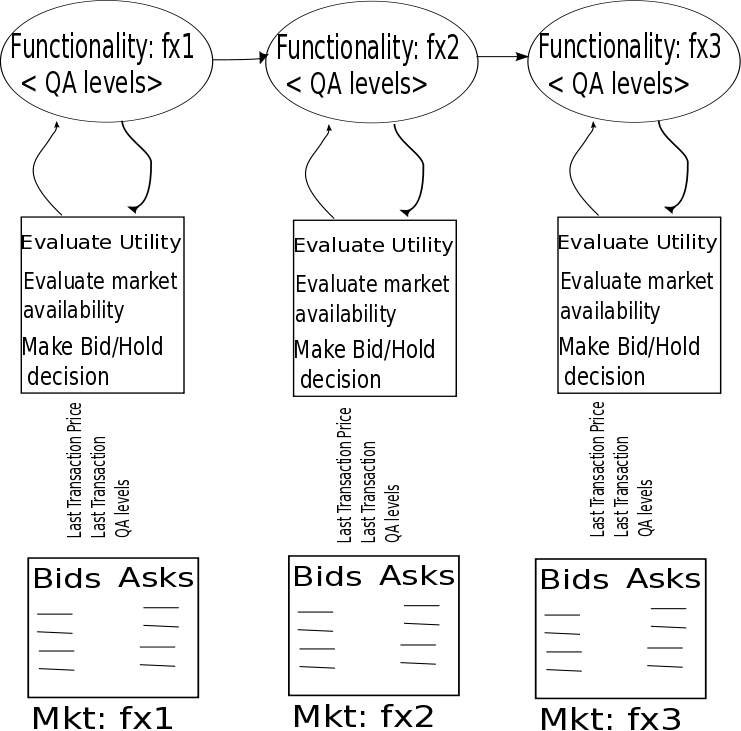
\includegraphics[width=3in, height=3in]{drawings/buyers-and-market.png}
  \caption{Web-services with agents that decide when to approach the market}
 \label{marketplace}
%   \end{minipage}
 \end{figure}
  


%We populate several markets with buying agents and selling agents. As mentioned before, each abstract service ($f_{x}$) is sold in a market that is specific to $f_{x}$. All the buying agents and selling agents in this market, trade web-services that deliver $f_{x}$ in functionality. We assume that there exists a market for every $f_x$, that is needed.  

\subsubsection{QoS constraints}
For any application, it is not enough to have functionality. Rather, it requires to exhibit a certain QoS that determines whether it is acceptable to the user or not. For e.g., given a video-library sorting service, it is not enough to sort videos correctly but it must also sort fast enough for the user's purposes. Depending on the specific user, this expectation of performance will vary. It is this variation in expected QoS that we aim to self-adapt to. Now, the QoS exhibited by an application composed of services, is a function of the QoS exhibited by each of its constituent services. The selection of concrete services must therefore be guided by the QoS constraints that are contingent upon the entire application. We consider the following types of QoS constraints on the application:
\begin{enumerate}
\item One-of-list constraint: This type of constraint refers to QoS attributes that usually occur in the domain as a list of options. For e.g., encryption options such as SHA-128, SHA-256, Blowfish, Serpent, etc.
\item Exactly-this constraint: This type of constraint refers to QoS attributes which are available at discrete levels. For e.g., bandwidth options like 1 mbps, 2 mbps, 10 mbps, 20 mbps.
\item More-than constraint: With this type of constraint, the application seeks to maximize the value obtained in that QoS attribute domain. For e.g., reliability, performance, reputation. In this type of constraint, the value specified is a lower bound and even if a service does not deliver \textit{at least} the minimum specified level of constraint, then it cannot be considered for composition.
\item Less-than constraint: With this type of constraint, the application seeks to minimize the value obtained. For e.g., cost. Similar to the previous constraint, if a service does not meet the constraint specified, then it cannot be considered for composition.
\end{enumerate}
These constraints are applied in the evaluation of services. Ranking amongst the services is done via calculation of utility that is calculated via the following rules:
\begin{enumerate}
\item The one-of-list and exactly-this constraints are boolean constraints, \textit{i.e.,} achieving these constraints results in a utility of exactly $1$ or $0$ (if not achieved). 
\item More-than constraints and Less-than constraints (also called positive and negative constraints in \cite{Ardagna2007Adaptive}) are evaluated as in \cite{Ardagna2007Adaptive}: 
\hspace{1cm}
\begin{table}[h]
\begin{tabular}{|p{1cm}p{5cm}|}
\hline
More-than & \[ \omega = \frac{QoS_{This} - QoS_{MinAvl}}{QoS_{MaxAvl} - QoS_{MinAvl}} \] \\
\hline
Less-than & \[ \omega = \frac{QoS_{MaxAvl} - QoS_{This}}{QoS_{MaxAvl} - QoS_{MinAvl}} \] \\
\hline
\end{tabular}
\end{table}
\end{enumerate}

\subsubsection{Structure of Workflow}
The end-to-end QoS exhibited by an application also affected by the structure of the workflow. Depending on how services are composed, the contribution of an individual concrete service to the overall QoS might be great or small. In figure \ref{composition_types}, we see the different basic structures that an application workflow might use. 

 \begin{figure}
 %  \begin{minipage}[b]{0.4\linewidth}
     \centering
     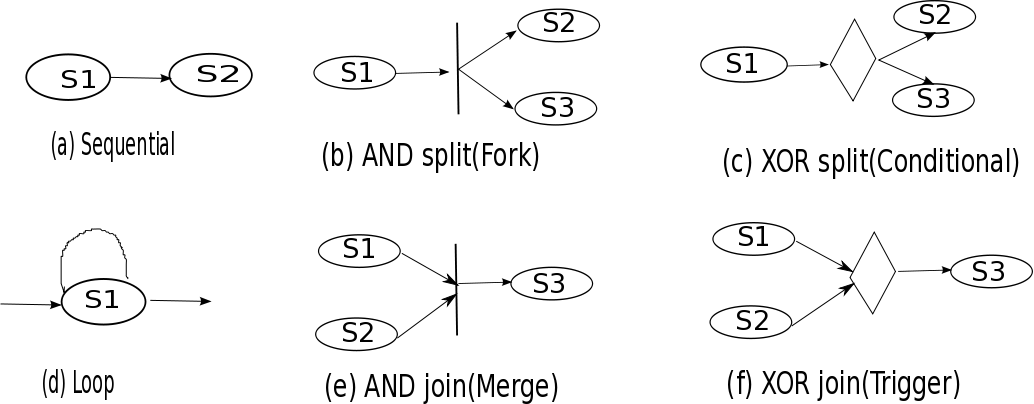
\includegraphics[width=3in, height=3in]{drawings/composition_types.png}
   \caption{Types of service composition}
  \label{composition_types}
 %   \end{minipage}
  \end{figure}

The end-to-end QoS that the application experiences is influenced to a large extent by its structure. In \cite{Cardoso2004Quality}, Cardoso et al. describe Stochastic Workflow Reduction (SWR), a recursive method for calculating the end-to-end QoS, based on the individual services' QoS values as well as the structure of the application. We use SWR as our mechanism for evaluating whether the individual QoS of the services satisfies the application's constraints. 

\subsubsection{Buyer}
The Buyer is a trading agent that buys a web-service for an Application, \textit{i.e.,} it trades in a market for a specific $f_x$. Each web-service, available in $f_x$, exhibits the same QoS ($\omega \in QoS$). The only differentiating factor is the degree to which that is exhibited  ($ \omega_{i} \in \mathbb{R}_{0}^{1} $). Hence, if an application has $K$ QoS that it is concerned about, then the QoS that it gets for each of the $f_{x}$ that it buys is:
	 \begin{equation}
	  \Omega^{f_{x}} = \langle \omega_{1}^{f_x}, \omega_{2}^{f_x}, \omega_{3}^{f_x}, \ldots, \omega_{K}^{f_x} \rangle \label{eq:exhibited_qa}
	 \end{equation}

The amount that the buyer is prepared to pay is called the \textsl{bid price} and this is necessarily \textit{less than or equal to} the $B_{f_x}$, where $B_{f_x}$ is the budget available with the buyer. The combination of $\Omega$ demanded and the \textsl{bid price} is called a \textsl{Bid}.

\subsubsection{Seller}
Each seller is a trading agent, selling a web-service that exhibits the QoS required in (\ref{eq:exhibited_qa}). The degree to which each qa($\omega$) is exhibited in each $f_x$ being sold, is dependent on the technological and economic cost of providing it. For example, if the cost of providing $f_x$ with $\Omega = \langle 0.5, 0.6 \rangle$ is low, then there will be many sellers providing $f_x$ with a low \textsl{ask price}. Conversely, if the cost of providing $f_x$ with $\Omega = \langle 0.8, 0.9 \rangle$ is high, then the \textsl{ask price} will be high. An individual seller's \textsl{ask price} can be higher or lower based on other factors like number of sellers in the market, the selling strategy etc. For the purpose of this paper, we consider only a single constraint between cost and \textsl{ask price}, where the \textsl{ask price} is always \textit{greater than or equal to} the cost. The combination of $\Omega$ and \textsl{ask price} is called the \textsl{Ask}. Every service is sold for a pre-specified $n$ calls, \textit{i.e.,} a purchase of a service entitles the buyer to make $n$ (market specified) calls to that service. Provenance regarding the actual usage of the service, can be easily established through the use of authentication keys, etc. 

\subsubsection{Market} 
A market is a set of buyers and sellers, all interested in the same functionality $f_x$. The factors differentiating the traders are:
	\begin{itemize}
	 \item \textbf{$\Omega$:} The combination of $\langle \omega_{1}, \omega_{2}, \ldots \omega{k}\rangle$
	 \item \textbf{\textsl{Price:}} Refers to the \textsl{bid price} and \textsl{ask price}. The buyers will not pay more than their respective \textsl{bid price} and the sellers will not accept a transaction lower than their respective \textsl{ask price}. 
	\end{itemize}

The mechanism of finding a matching buyer-and-seller is the \textit{continuous double auction}(CDA). A CDA works by accepting offers from both buyers and sellers. It maintains an orderbook containing both, the \textsl{bids} from the buyers and the \textsl{asks} from the sellers. The bids are held in descending order of price, while the asks are held in ascending order, \textit{i.e.}, buyers willing to pay a high price and sellers willing to accept a lower price are more likely to trade. When a new \textit{bid} comes in, the offer is evaluated against the existing \textit{asks} in the book and a transaction is conducted when the price demanded by the \textit{ask} is lower than the price the \textit{bid} is willing to pay \textbf{and} all the QoS attributes in $\Omega$ of the ask are \textit{greater than or equal to} all the QoS attributes in the $\Omega$ of the \textit{bid}. After a transaction, the corresponding \textit{bid} and \textit{ask} are cleared from the orderbook.
\begin{figure}
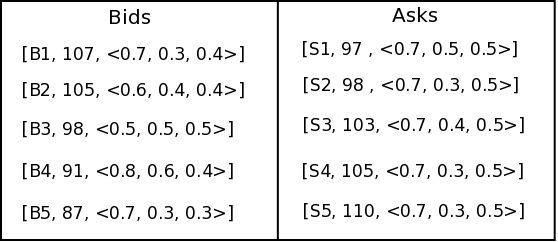
\includegraphics[scale=0.31]{drawings/orderbook.png}
\caption{Orderbook at time $t_{0}$}
\label{orderbook}
\end{figure}
Figure \ref{orderbook} shows the state of the orderbook at some time \textit{$t_{0}$}. Maximizing the number of transactions would lead to a possible set like: $[B1-S4, B2-S3, B3-S1]$. Calculating this optimal set, however, quickly becomes infeasible as the number of bids and asks increase, since the number of pairwise comparisons needed increases exponentially.  With a CDA, the set of transactions is: $[B1-S1, B2-S3]$. This is so because a CDA evaluates bids and asks, as they come in and the first possible match is set up as a transaction. Thus, $[B1-S1]$ is immediately matched and removed from the orderbook, and then $[B2-S3]$ is matched.  Since this procedure is carried out for every offer (\textit{bid/ask}) that enters the market, the only bids and asks that remain on the orderbook are those that haven't been matched (figure \ref{orderbook-after-one-pass}). This procedure is much faster, and easily parallelizable. Although counter-intuitive, it has been shown that even when buyers and sellers have Zero-Intelligence, the structure of the market allows for a high degree of allocative efficiency \cite{Gode1993Allocative}. Zero-Intelligence refers to a strategy, where the agents involved, do not consider any historical information about trades, and nor do they possess any learning mechanism. Thus, Zero-Intelligence marks the lower limit of the efficiency of a CDA market.
\begin{figure}
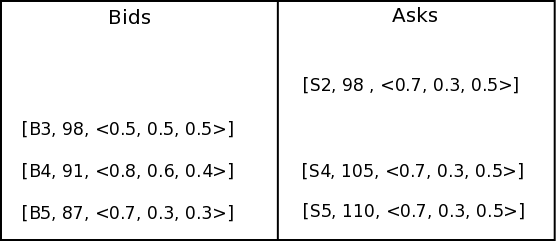
\includegraphics[scale=0.31]{drawings/orderbook-after-one-pass.png}
\caption{Orderbook at time $t_{1}$}
\label{orderbook-after-one-pass}
\end{figure}

%TODO: INSERT MODIFIED CDA: 2-STEP: 1 FOR TRADING AND 2 FOR APP TO CALCULATE BEFORE COMMITMENT. REFERENCE RAMCHURN'S PAPER ON 2-STEP CDA FOR EVIDENCE OF BETTERNESS

\subsubsection{Applications}
The Application is a composition of services from different markets. At the agent-level, the application agent communicates with each of the buying agents ($f_{x} \in F_{x}$) and communicates a budget ($B_{f_{x}}$). The buyer then initializes itself with a random $\Omega^{f_x}$ and starts trading. The adaptation occurs through the revision of bids, that happen after each round of trading. After each round of trading, depending on the $\Omega$ obtained by the buyer, the Application has procured a total QoS that is calculated, using Stochastic Workflow Reduction\cite{Cardoso2004}.\\
Buying and using a web-service involves many costs, and these must be compared against the projected utility gain to decide whether it is worthwhile to switch. These may be enumerated as:
	\begin{itemize}
	 \item \textit{Buying Cost:} The price of purchasing the web-service for \textsl{n} calls ($p_{f_x}$)
	 \item \textit{Transaction Cost:} The amount to be paid to the market, for making the transaction ($t_{f_x}$)
	 \item \textit{Switching Cost:} Every contract with a web-service would incorporate the total number of calls or the time for which the service is available, at the transaction price. If the application wants to break this contract, it would have to pay a penalty to the supplier. This amount of penalty to be paid is the switching cost ($s_{f_x}$). In real life, the switching cost would include other variables like opportunity cost, penalties levied by the application's consumers for loss of service, etc. Since these are more difficult to measure, we restrict ourselves to the directly observable values, such as penalty for breaking a contract.
	 \end{itemize}
Thus, the total cost that the application must consider is:
	\begin{equation}\label{eq:total_cost} 
	 TC_{f_x} = p_{f_x} + t_{f_x} + s_{f_x}
	\end{equation}
	 
We assume that, for every application there exists a function that maps $TC_{f_x}$ to an equivalent $\Omega^{f_x}$. The application could easily buy the best possible web-service(s) available, if it was prepared to spend a large amount of money. However, in reality, every application is constrained by a budget($B$) that it is willing to spend. The application apportions budget as well as QoS constraints to each of its constituent buyer agents (see algorithm \ref{Initialization}).

%Allocating $B$ amongst the functionalities that it is buying ($f_x \in F_x$) is a matter of strategy and/or the relative importance of each $f_x$. 
%	\begin{equation}
%	 \forall f_{x} \in F_{x}, \sum B_{f_x} = M 
%	\end{equation}

%After every round, the application compares the privately known $\Omega_{f_x}$ with the $\Omega^{b}_{f_x}$ and determines whether to punish/reward the buyer. From this piece of information, the buyer can only guess whether it needs to improve the $\Omega^{b}_{f_x}$ that it obtained or the price that it paid. Once the  $\Omega^{b}_{f_x}$ is close enough to the private $\Omega_{f_x}$, then the application refrains from trading any further, until it changes the privately known $\Omega_{f_x}$. Changing of the private $\Omega_{f_x}$ simulates the change in the environment, which has prompted adaptation by the application. The buyers have to now re-approximate the private $\Omega_{f_x}$.
Traditionally, a CDA works on a single piece of information, price. However, we modify the bids and asks to be multi-attribute, \textit{i.e.,} each bid also contains the minimum QoS levels that the buyer wants and each ask contains the maximum QoS levels that the seller is willing to provide. Thus, a transaction between a buyer and a seller is now an agreement to provide a certain functionality, at a certain price, at pre-defined QoS levels.
%After every round of trading, the application calculates the total utility that it obtained after the trades and compares it to the previous utility it had. Depending on whether the utility in the current round is better or worse, the application provides an appropriate feedback to all the buying agents. This allows an agent to realize the effect of its action on the overall utility. It then modifies its bid, accordingly.

In Figure \ref{marketplace}, we see the functionality being composed at the top and the agents below calculating the utility achieved by each trade. The agents are also able to observe the last known transaction price and QoS levels in their markets. This allows them to create bids, that are most likely to result in a trade.

\begin{algorithm}
 \DontPrintSemicolon
 \KwData{Total budget available for entire application}
 \KwResult{All agents initialised and ready to trade}
 \Begin{ 
 \ForEach{$Agent\ a$}{
 	Find list of markets $(M)$ corresponding to $a_{f_{x}}$\;
 	Choose $m \in M$\;
 }
 \ForEach{$Agent\ a$}{
 	Register in $m$\;
 	$a \longleftarrow m_{medianTransactionPrice}$\;
 	$a \longleftarrow m_{medianQoS}$\;
  }
  Apply SWR $\longleftarrow \langle \omega_{f_{1}}, \omega_{f_{2}}, \omega_{f_{3}} \ldots \rangle$\;
  \eIf{$constraintsMet$}{
	 \ForEach{$Agent\ a$}{
     	$a_{budget} \propto a_{medianTransactionPrice}$\;
	    $a_{minQoSlevel} \longleftarrow a_{medianQoS}$\;
  	}  	
 } {
  	Choose different $m$\;
  	\If{$allMarketsExhausted$}{
  		TerminateWithFailure\;
  	}
  }
 }
 \caption{Initialization of Agents}
 \label{Initialization}
\end{algorithm}

\begin{algorithm}
 \DontPrintSemicolon
 \KwData{$I \longleftarrow \mid set\ of\ web-services\ that\ are\ the\ input \mid$}
 \KwData{$O \longleftarrow \mid set\ of\ web-services\ that\ are\ the\ output \mid$}
 \KwData{$\Upsilon \longleftarrow ElectedHead$}
 \Begin{
 		\ForEach{$Agent\ a$}{
 				
 				Create bid with {
 						$a_{bid^{QoS}} \geq a_{minQoSlevel}$\;
 						$a_{bid^{price}} \longleftarrow random(a_{budget})$\;
 				}
 				
 				$m \longleftarrow register(a_{bid})$\;
				$a \longleftarrow wait(m_{trading\_round})$\;
 				\eIf{trade}{
 						$a_{utility} \longleftarrow \alpha(QoS_{a}) + \beta(QoS_{I}) + \gamma(QoS_{O})$\;%
						$Communicate(\Upsilon \longleftarrow a_{utility})$\;
						$Communicate(\Upsilon \longrightarrow a_{feedback})$\;
						\eIf{$\mid$$a_{feedback}\mid\ \leq \epsilon$}{
							$a\rightarrow StopTrading$\;
						}{
							$a\rightarrow ReviseBid$\;
						}
 				}{
 						$a_{utility} \longleftarrow negative(a_{minQoSLevel})$\;
 						$a_{notrade}++$\;
 						\If{$a_{notrade} == k$}{
 								$a_{nextCommunication} \longleftarrow InsufficientBudget$\;
 						}
 				}
 		}
 }
 \caption{Adaptation by Buying Agents}
 \label{Adaptation}
\end{algorithm}


% \begin{algorithm}
%   \KwData{$Neighbour \in \{I,O\}$}
%   \Begin{
%   	\ForEach{$Agent\ a$}{
% 		Gossip($a\leftarrow Neighbour_{nextCommunication}$)
%  		\If{$Neighbour_{nextCommunication} == InsufficientBudget$}{
%  			$a \rightarrow InspectBudget$\;
%  			\eIf{$a \rightarrow HasSurplus$}{
%   				$a_{apportionedSurplus} \rightarrow Neighbour$\;
%  			}{ 
%  				$a_{nextCommunication} \leftarrow 'Insufficient Budget'$\;
%  			}
% % 			
%  		}
%  	}
%  }
%   \caption{Re-allocating Resources}
%   \label{Reallocation}
% \end{algorithm}

\subsection{Utility Function}
A utility function is used to evaluate the QoS obtained by buying a particular web-service. This is done by mapping the QoS values advertised by the web-service onto real values. This involves scaling the QoS values onto a uniform scale, and then applying any weights that the application might indicate as its preference. This mechanism enables QoS attributes that are measured in different units to be treated identically, while calculating utility. Each QoS attribute has a different function, to calculate the end-to-end value. For e.g., while calculating the end-to-end value of performance, we use:
	\begin{equation} 
		App_{performance}  = Min_{i \in {1..n}}(a_{i}^{performanceQoS})
	\end{equation}
whereas availability is calculated as: 
	\begin{equation}
		App_{av} = \prod_{i=1}^{n}(a_{i}^{av})	    
	\end{equation}
Thus, in a certain configuration, an application could potentially meet one of its target QoS, while not meeting another. The utility function must be able to reflect this. We use the \textit{Simple Additive Weighting} from \cite{Yoon1995Multiple} for this purpose.  For each application, the target level of QoS is also mapped onto a real value, that is designated as the ideal utility level (IUL) for that application. 

\subsection{Calculating Achieved QoS and Feedback}
 The application agent collects information from each of its buyer agents and calculates the cumulative QoS. It then compares the achieved cumulative QoS against the targetted QoS. On a per-QoS attribute basis, the difference between the achieved and the targetted, is computed and communicated back to the buyer agents.  Intuitively, the easiest way to calculate the application's cumulative QoS is through a central agent that collects QoS information, from each of the buying agents. However, this would lead to dependence on a centralized agent and thus become a bottleneck, in case of applications with a large number of services. We use a gossip-based algorithm, much like Push-Sum\cite{Kempe2003Gossip-Based}, to communicate QoS values. However, unlike Push-Sum, we make the agents gossip information, only to their neighbours' agent (see algorithm \ref{Communication}). A neighbour is defined as a service that is either in the input set or the output set, of a particular service. After each round of gossiping, each agent accumulates its neighbour's QoS information into the QoS calculation function. In the next round of gossip, it sends the new information to other neighbours. Each agent tags its QoS information with its name. This allows agents to recognize if they've seen/sent a particular message before. Agents only send out information that they haven't sent before. When an agent recognizes that it has received all QoS information from all other agents, it runs utility calculation procedures. Feedback is calculated as the difference between the obtained utility and the IUL. The feedback indicates not only the magnitude of the difference, but also the direction. That is, whether the buyer agents have undershot or overshot the target QoS.   
	
\begin{algorithm}
 \KwData{$Neighbour \in \{I,O\}$}
 \Begin{
 	\ForEach{$Agent\ a$}{
	 	\While{ Not received from all agents}{
			Communicate($Neighbour \longleftarrow a_{QoS}$)
		}
		$a_{utility} \longleftarrow CalculateTotalUtility(\Upsilon)$\;
		\eIf{$a_{utility} \pm \epsilon IdealUtility$}{
			$a \leftarrow StopTrading$\;
		}{
			$a \leftarrow Feedback$\;
		}
	}
 }
 \caption{Communicating Achieved QoS}
 \label{Communication}
\end{algorithm}

\subsection{Adapting Bids and Asks}
Bids and Asks form the core of the adaptive process of our mechanism. After an initial start that is influenced by the current QoS values and prices in the market, the buyer agents perform the equivalent of a local search, by means of adjusting the QoS values in their bids. There are many ways to calculate the new QoS value, given a current value and the feedback. We use the least mean squares method (also known as \textit{Widrow-Hoff learning rule})\cite{Haykin2003Least} to adapt the QoS and the price. We use ZIP\cite{Cliff1998Simple}, a fairly simple improvement on the Zero-Intelligence algorithm, that implements the Widrow-Hoff learning rule to perform a gradient descent of the current price (in the ask or bid) to the last transaction price, in the market.  Also, depending on the feedback by the application, each individual buying agent either increases or decreases the QoS attribute values, that it is bidding for. The increase or decrease is determined by the direction indicated in the feedback. The magnitude of change is more difficult to realize. The magnitude indicated in the feedback is a cumulative figure, referring to the difference between target and achieved levels of QoS, for the application. Therefore, each agent changes its QoS bid attributes by a fraction of the magnitude indicated in the feedback (see algorithm \ref{bid_revision}). We use a simple average (magnitude of feedback divided by number of agents in the workflow) to calculate this fraction.\\
Selling agents also modify their asks, in order to get a better deal for their services. If an agent is able to trade, it increases the price it charges, in the next ask. The sellers also use ZIP to decide on the new charging price(see algorithm \ref{ask_revision}). If the seller is unable to find buyers at a higher price, it drops back to its older price. If it is still unable to find a buyer, then it goes back to the original ask that enabled the agent to transact.\\
The buyers are constrained by their budget, for the prices that they're willing to pay. The sellers are also constrained by their actual QoS values that they can provide.
 
 \begin{algorithm}
 \DontPrintSemicolon
  \KwData{$a_{feedback}, last\_transaction\_price\ in\ m$}
  \Begin{
  	\eIf{$a_{traded}$}{
		$direction, magnitude \leftarrow split(a_{feedback})$\;
		\eIf{$direction == 'Increase'$}{
			$a_{newbid^{QoS}} \leftarrow Increase(a_{bid^{QoS}},magnitude)$\;
		}{
			\eIf{$direction == 'Decrease'$}{
				$a_{newbid<QoS>} \leftarrow Decrease(a_{bid<QoS>},magnitude)$\;
			}{
				$a\rightarrow StopTrading$\;	
			}
		}
	}{
		\eIf{$a_{notrade} == k$}{
			$a_{nextCommunication} \leftarrow 'Insufficient Budget'$\;
		}{
			$a_{bid<price>} \leftarrow ZIP(last\_transaction\_price)$\;
		}
	}
  }
  \caption{Revising a Bid}
  \label{bid_revision}   
 \end{algorithm}

\begin{algorithm}
 \DontPrintSemicolon
  \KwData{$last\_transaction\_price\ in\ m$}
  \Begin{
  \ForEach{$SellingAgent\ a$}{
  	\eIf{$a_{traded}$}{
	    $a_{newask<price>} \leftarrow ZIP(Increase, a_{ask<price>}, last\_transaction\_price )$\;
	}{
	    $a_{newask<price>} \leftarrow ZIP(Decrease, a_{ask<price>}, last\_transaction\_price)$\;
	}
  }
  }
  \caption{Revising an Ask}
  \label{ask_revision}   
 \end{algorithm}
 
\subsection{Stopping Criteria}
Trading by the agents (and hence adaptation) stops when the application has reached its IUL. Depending on the domain, the application may decide to tolerate a small ($\epsilon$) level of deviation from the IUL. Thus, a satisfactory zone of QoS values is reached which is acceptable to the application. The level of tolerance can be made arbitrarily small or even zero. The stopping criteria can be different for different applications, and indeed, has no restriction whatsoever. Clearly, if it is set injudiciously, the application may either stop adapting too quickly or may never stop adapting. Thus, it becomes an important parameter to tune.

\subsection{Re-starting Conditions}
There are two conditions where an application that has already reached a satisfactory level of QoS, needs to start adapting again:
	\begin{enumerate}
	    \item Internal Stimulus: When a QoS violation is detected at any of the web-services, the application needs to re-start its search for a new web-service to replace the old one. This is not an application-wide adaptation, but localised to a particular web-service
	     \item External Stimulus: When the application's end-to-end QoS target changes, the application triggers an adaptation in each of its web-services, whereby all the trading agents go through the trading process again, until the stopping criteria is met
	\end{enumerate}
Both these events occur at different time scales. The internal check for QoS violation is a continuous check and concerns itself with performance of the web-service across relatively shorter periods of time. The external stimulus, on the other hand, typically happens when budgets for operation change drastically or external events cause change in performance or reliability requirements. This happens at relatively rarer intervals. This implies that once an application reaches close to its desired level of QoS, most of the buying agents stop trading.\\
\textbf{QoS Monitoring}: Monitoring a web-service for an SLA violation is a topic of research in its own right. There have been several attempts in this direction, most notably from \cite{Chau2008Automatinga, Michlmayr2009Comprehensive, Raimondi2008Efficient} and \cite{Skene2004Precise} In this paper, we do not attempt to devise our own scheme for QoS monitoring. Rather, we assume that one of the methods outlined in the afore-mentioned research, is used. 

\subsection{Scalability Requirements for Dynamic Web-Service Composition}
In none of the papers that we surveyed (in section \ref{dynamic_wsc}), did we find a single rigorous definition of what it would mean for a dynamic service composition technique to be scalable . In the absence of such a definition, it is difficult to judge, whether a technique is really scalable or not. To alleviate the problem of capricious definitions of scalability, we use a definition of scalability from \cite{Duboc2007framework}: \textit{a quality of software systems characterized by the causal impact that scaling aspects of the system environment and design have on certain measured system qualities as these aspects are varied over expected operational ranges}.\\
According to \cite{Duboc2007framework}'s definition, when these variables change, they have an impact on the system's qualities. In our case, the system qualities that we want to measure are:
	\begin{enumerate}
		\item Efficacy, measured as a fraction of the total applications that are able to achieve their required QoS
		\item Performance, measured as the amount of time taken to select services, when critical variables vary over an expected range.
	\end{enumerate}	 
After a careful perusal of available literature on dynamic web-service composition, we have determined that the following variables are critical, in their effect on the performance of the service selection technique. We explicate the critical variables of the system as:
	\begin{enumerate}
		\item Tasks per workflow, \textit{i.e.}, the number of abstract services in a workflow
		\item Number of candidate services, \textit{i.e.}, the number of concrete services available per abstract service
		\item Number of QoS values per candidate service
	%	\item Number of end-to-end QoS constraints
%		\item Number of markets available for acquiring concrete services
	\end{enumerate}
	
Eliciting the 'normal' operational range of these variables is an involved task, and outside the scope of this paper. Instead, we consider the ranges of variables, based on a study conducted by Cloud Harmony \cite{2011CloudHarmonyStudy}. The ranges that we consider, are shown in table \ref{scaling_range}:
%\begin{center}
\begin{table}
\begin{tabular}{|c|c|}
\hline
\textbf{Variable} &  \textbf{Range} \\ \hline
Tasks-per-Workflow & 10 -- 100 \\ \hline
Candidate-Services & 1 -- 10 \\ \hline
Number-of-QoS & 1 -- 5 \\ \hline
%End-to-end Constraints & 1 -- 10 \\ \hline
%Number-of-Markets & 1 -- 5 \\ \hline
\end{tabular}
 \label{scaling_range}
 \caption{Operational range of service parameters}
\end{table}
%\end{center}

\subsection{Design and Implementation}
%In \citep{Cheng2009}, the authors comment on the engineering challenges of building a self-adaptive system, and emphasize the fact that the %feedback loop is of utmost importance. 
The design of our implementation is based on the publish-subscribe architectural style. This style was chosen for its decoupling properties, such that each communicating entity in the system is independent of every other. This fits in well, with our notion of agents acting on the basis of their own goals and their environment, in a decentralized manner. Each type of agent described previously, is both an event publisher and an event subscriber. That is, each application agent generates events that describe when the application's QoS constraints have changed, when the budget has changed, etc. These events are subscribed to, by the buyer agents that belong to that application. The buyer agents, for their part, publish events relating to the market that they're registered with. Similarly, the market agents publish events relating to the start of trading, transaction events, etc. The event-based paradigm fits well with the QoS monitoring schemes, as well. Both \cite{Zeng2007Monitoring} and \cite{Michlmayr2009Comprehensive} use events to monitor and communicate SLA violations. \\

\begin{figure}[ht]
	\centering
	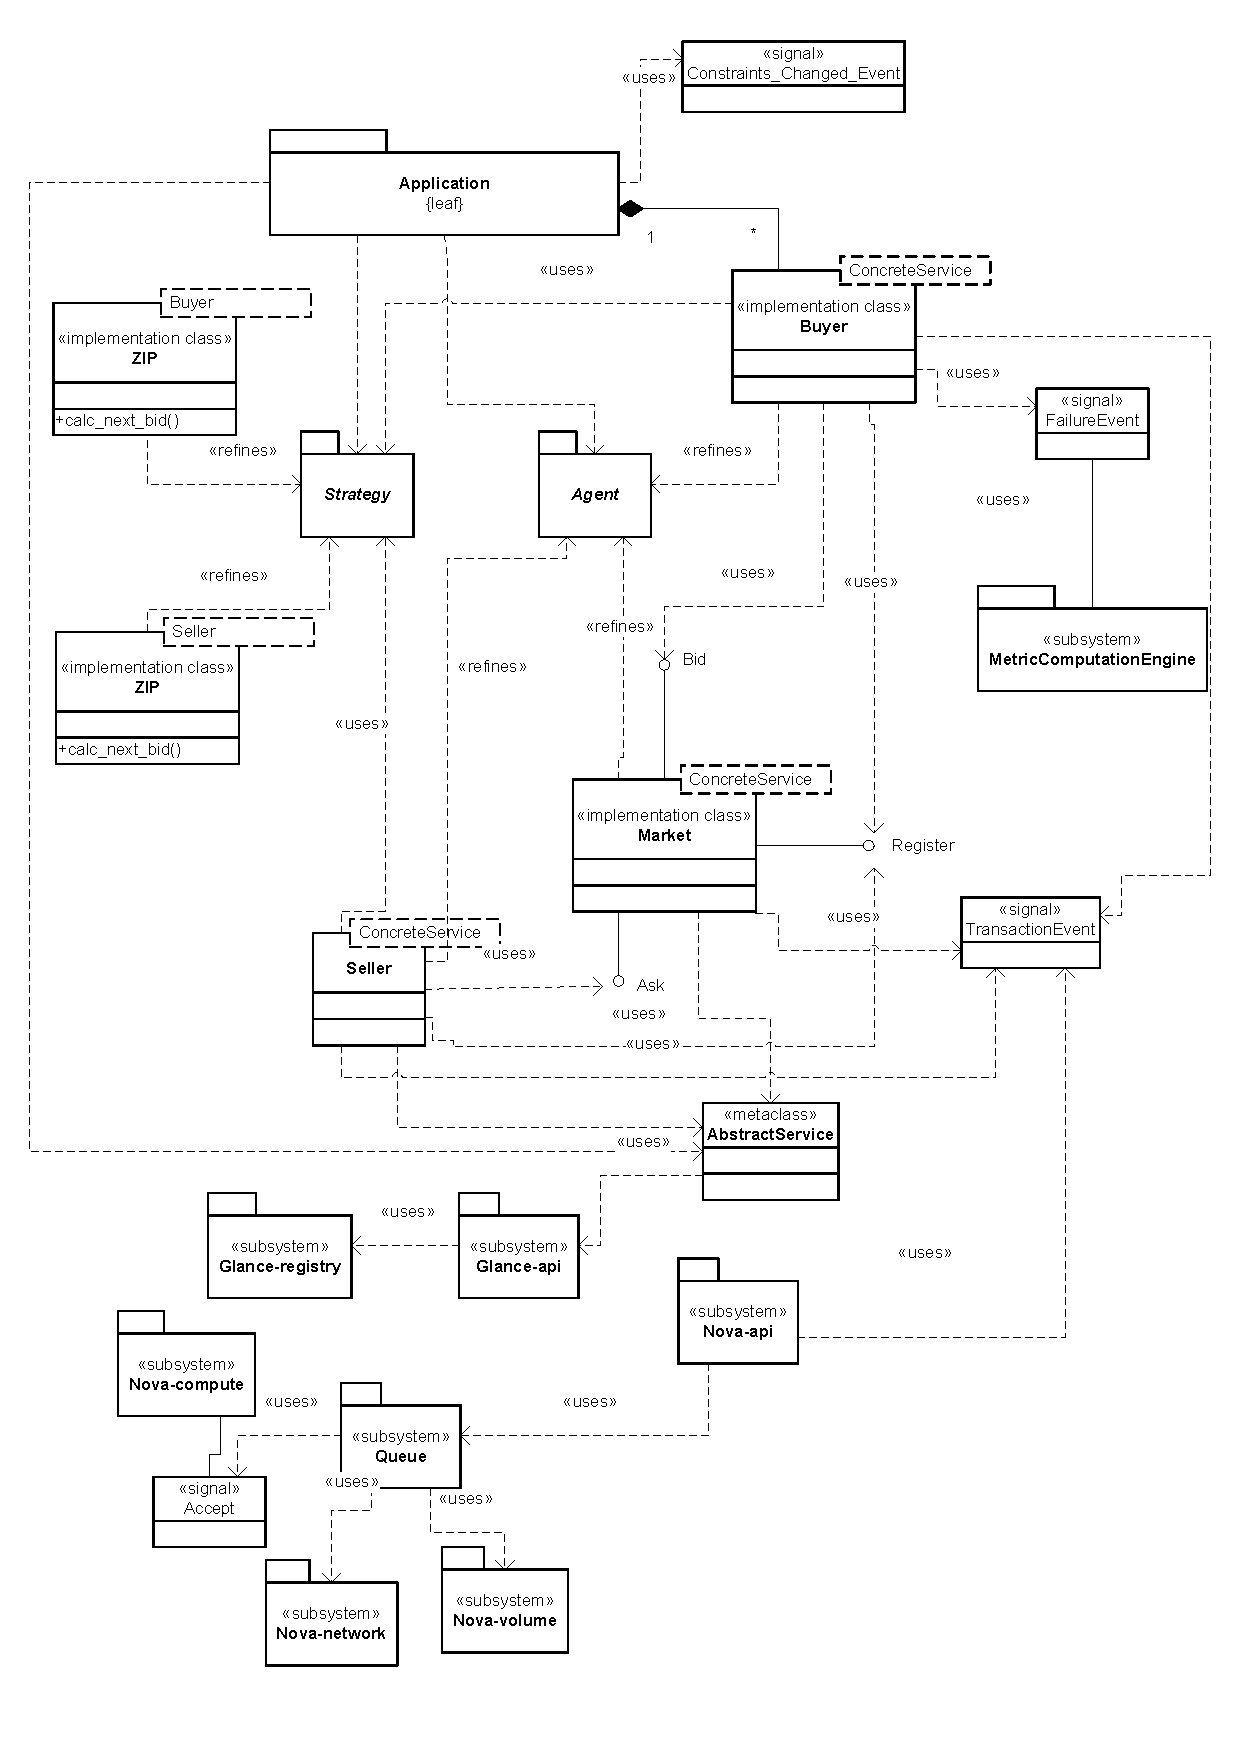
\includegraphics[trim = 30mm 50mm 50mm 30mm, clip, totalheight=0.50\textheight, width=0.45\textwidth]{drawings/class_and_package_diagram.pdf}
	\label{class_diagram}
	\caption{Simplified class diagram of core entities}
\end{figure}

In figure \ref{class_diagram}, we show a simplified class diagram of the main entities of the system. Each entity subscribes to, and publishes events through the use of sockets. In the figure, we show "Metric Computation Engine" as a black-box that generates events relating to SLA violations by services. The buyer agents listen to these events to decide whether to initiate an adaptation or not. The market agent listens to these very same events, to adjust its reliability ratings of each service. In figures \ref{setup_phase} and \ref{trading_phase}, we show the sequence of messages passed between the agents in AUML. \\

\begin{figure}
	\centering
	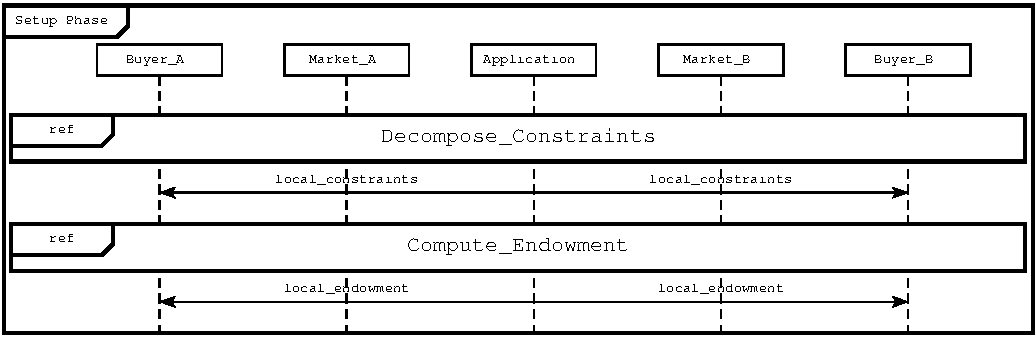
\includegraphics[scale=0.6]{drawings/setup_phase.pdf}
	\label{setup_phase}
	\caption{Sequence of messages during the initial setup phase}
\end{figure}

\begin{figure}
	\centering
	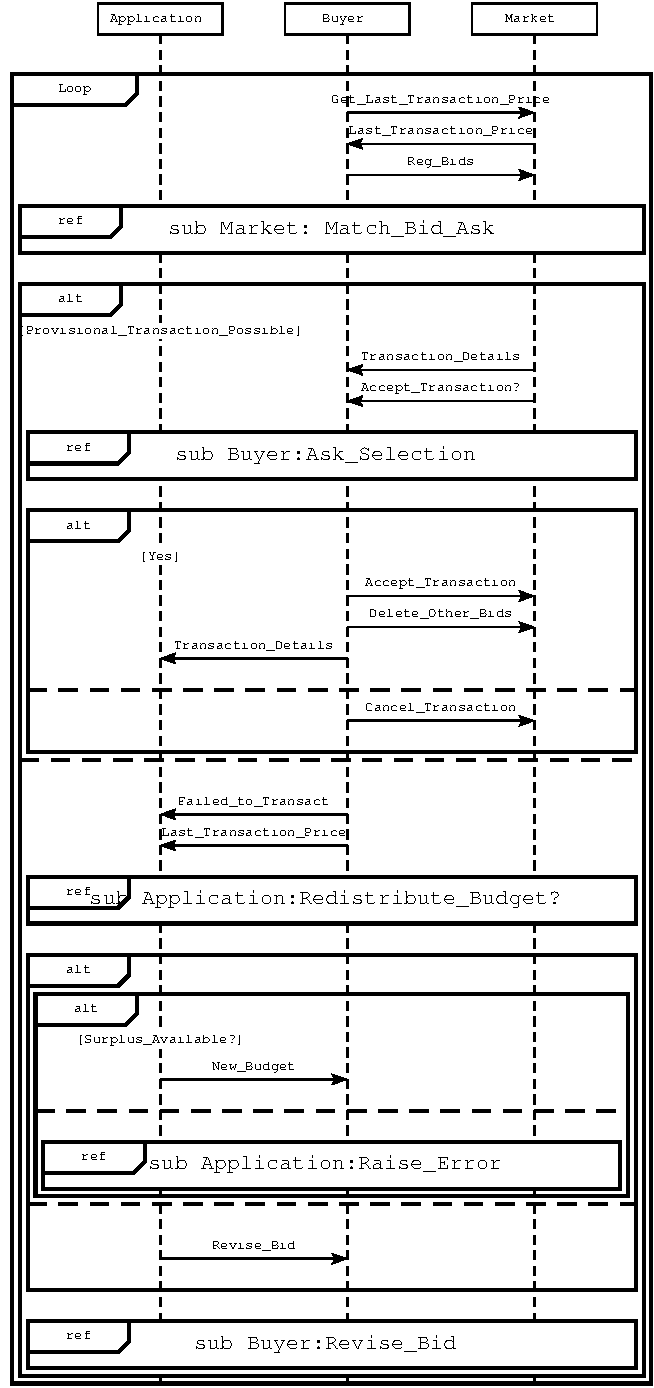
\includegraphics[scale=0.6]{drawings/trading_phase.pdf}
	\label{trading_phase}
	\caption{Sequence of messages during trading}
\end{figure}


\textbf{Implementation of double auction}: The most computationally intensive aspect of the entire system is the implementation of the double auction mechanism. Storing the bids and asks as simple lists results in a huge amount of searching for matching purposes. We modify the 4-heap data structure, as suggested in \cite{Wurman1998Flexible}, to store our multi-attribute bids and asks. In our python implementation, we use the heapq module to store bids in a descending order and asks in an ascending order. This decision allows for bids that are willing to pay a higher price, get matched first. 

\section{Evaluation}
\subsection{Empirical Study}
%Consider a company that specializes in providing 3D rendering services. To save on capital expenditure, it creates an application that lives on the cloud and uses web-services to do the actual computation. This allows it to scale up and scale down the number of computational nodes, depending on the size of the job. However as business improves, the company implements a mechanism for automated submission of jobs, with differentiated rates for jobs with different priorities, requirements and even algorithms. For instance, a particular job may require texture and fluid modelling with a deadline of 30 hours, while another might require hair modelling with a tighter deadline of 6 hours. Yet another job might require ray-tracing with a deadline of 20 hours.
Consider a company that provides data-mining services. To take advantage of the elastic nature of demand for their services, they decide to construct an application that is composed of web-services from several clouds. That is, it leases storage space, computing power, sorting algorithms, visualizers and plugs-in its own data-mining algorithms, to provide an end-to-end service to its clients. Obviously, it is best able to make a profit, when it does not have to keep storage or other infrastructure idle. This prompts the company to create an application that self-adapts to the job in hand, and uses web-services with QoS levels dependant on the budget of the client. Consider other companies that provide other services, such as 3D rendering or game-world creation. Depending on the nature of the job, a texture modelling algorithm may be required or a fluid modelling service might be pressed into service with a deadline of 30 hours, while yet another involving hair modelling might be on a tighter deadline of 6 hours. This means that the application would need to change its \textit{performance QoS} dynamically. Depending on the kind of data and algorithm being used, the application's storage requirements would change as well. For certain tasks, the application might require large amounts but slow-speed storage, while others might require smaller amounts but higher-speed storage. These companies would like to be in an environment that allowed their applications to self-manage their QoS, depending on the business input that was provided, on a per-task basis. Each of these self-management decisions are constrained by the cost of change. The cost of change, in turn, would depend on factors like supply of desired service, availability, etc. 
 \begin{table}
 \begin{tabular}{| c | c | c | c | c |}
 \hline
 \small Abstract Svc & \small Concrete Svc & \small Perf & \small Avblty & \small Price\\ \hline
 \multirow{2}{*} {S1} 
 & $S1_{1}$ & 100 & 0.95 & 50\\
 & $S1_{2}$ & 180 & 0.92 & 66\\
 & $S1_{3}$ & 230 & 0.79 & 65\\
 & $S1_{4}$ & 170 & 0.73 & 90\\
 & $S1_{5}$ & 250 & 0.96 & 60\\ \hline
 
 \multirow{5}{*} {S2} 
 & $S2_{1}$ & 200 & 0.98 & 58\\
 & $S2_{2}$ & 150 & 0.93 & 80\\
 & $S2_{3}$ & 200 & 0.97 & 65\\ 
 & $S2_{4}$ & 170 & 0.93 & 82\\
 & $S2_{5}$ & 190 & 0.99 & 95\\ \hline
 
 \multirow{5}{*} {S3} 
 & $S3_{1}$ & 250 & 0.96 & 70\\
 & $S3_{2}$ & 240 & 0.91 & 50\\
 & $S3_{3}$ & 230 & 0.79 & 65\\ 
 & $S3_{4}$ & 150 & 0.73 & 80\\
 & $S3_{5}$ & 210 & 0.89 & 68\\ \hline
 
 \multirow{5}{*} {S4} 
 & $S4_{1}$ & 260 & 0.94 & 59\\
 & $S4_{2}$ & 225 & 0.91 & 60\\
 & $S4_{3}$ & 230 & 0.79 & 69\\ 
 & $S4_{4}$ & 180 & 0.73 & 80\\
 & $S4_{5}$ & 200 & 0.89 & 64\\ \hline
 
 \multirow{5}{*} {S5} 
 & $S5_{1}$ & 150 & 0.82 & 54\\
 & $S5_{2}$ & 140 & 0.71 & 49\\
 & $S5_{3}$ & 130 & 0.93 & 76\\ 
 & $S5_{4}$ & 120 & 0.73 & 81\\
 & $S5_{5}$ & 190 & 0.86 & 77\\ \hline
 
 \multirow{5}{*} {S6} 
 & $S6_{1}$ & 250 & 0.96 & 59\\
 & $S6_{2}$ & 230 & 0.91 & 73\\
 & $S6_{3}$ & 220 & 0.79 & 65\\ 
 & $S6_{4}$ & 170 & 0.73 & 90\\
 & $S6_{5}$ & 210 & 0.89 & 88\\ \hline
 
. & . & . & . & .\\ 
. & . & . & . & .\\
. & . & . & . & .\\
. & . & . & . & .\\ \hline

\hline
% \hline
 
\end{tabular}
\caption{Choice of services available}
\label{choice-of-services}
\end{table}
 
 In table (\ref{choice-of-services}), if a company wanted to optimize on Price, the set of selected services would be $[S1_{1}, S2_{1}, S3_{2}, S4_{2}, S5_{2}, S6_{1}]$. On the other hand, if it wanted to optimize on Performance, the selected services would be $[S1_{1}, S2_{2}, S3_{4}, S4_{4}, S5_{4}, S6_{4}]$. The calculations become more difficult if the optimizations need to be done on multiple QoS simultaneously, for e.g., Performance and Price or Performance and Availability. As the number of abstract services in the application's workflow increase, the number of combinations also increase correspondingly.
Another complication is that there is no way to precalculate the various alternative services available, in case of detection of QoS violation. This is due to the fact, that a service that was available at the time of calculation may no longer be available, at the same price and QoS configuration.\\
Consider a number of such companies operating on the cloud and dynamically optimising their applications. The cloud provider would like to ensure that the maximum possible number of services are used by these applications, since any unused service is a cost-burden on the cloud provider. In this scenario, our mechanism of self-adaptation achieves two objectives from both parties, applications and the cloud provider:
	\begin{enumerate}
	    \item providing a fast matching service based on price and QoS, and
	    \item allowing for high levels of matching 
	\end{enumerate}
\subsection{Methodology}
We simulate 300 applications, each application consisting of 10 abstract services trying to achieve their desired QoS levels, within a given budget. The budget that each application gets, acts as a constraint and the application's constituent trading agents (buyers) can never bid above their budgets. Each application generates a random level of QoS that it must achieve.\\
Once an application achieves its required QoS, it withdraws from trading until an internal or external stimulus occurs. An internal stimulus is when one of the concrete services exhibits a service violation. We model this violation by a small probability. An external stimulus occurs when the application decides to change its required QoS for any reason (say, a new job requires different QoS levels). This is simulated by using time as a parameter. Every application, once satisfied with its QoS, (as mentioned above) stops adapting. However, at some random time, every application receives a different job that requires different QoS levels. This prompts that particular application to adapt, and therefore, approach the market again.
 %, based on a study conducted by Cloud Harmony \cite{2011CloudHarmonyStudy}
% \subsection{Scalability}
% The scalability of a self-adaptive approach is slightly difficult to measure, since we're concerned not only with time and space complexity, but also with goodness complexity. 


\subsection{Results}
There are two perspectives from which to evaluate our mechanism, the individual application and the collective view of all applications present. We present both perspectives, with an emphasis on the collective view since it provides a better idea on the scalability of our mechanism. All simulations are reported as an average of a 100 simulations.\\
\subsubsection{Individual Perspective}
At the individual level, we measure the difference between the targetted QoS level and the QoS actually achieved by the application. If the difference is zero, then the application has managed to achieve the exact level of QoS required (ideal level). We also set a tolerance level, within a certain fraction of the target level. Once within this tolerance zone, agents stop adapting. Only the probability of internal stimulus causes the individual buyer agents to approach the market and buy a new service. In figure \ref{goodness} we see an average application's achievement of QoS levels. We see that the QoS achieved, initially starts out at a level much below the application's expectations, but it quickly manages to reach the tolerance zone. The only reason that the application doesn't exhibit a constant level of utility once it reaches the tolerance zone, is that random internal QoS violations cause it to seek new services to substitute for under-performing services. This causes the exhibited utility to fluctuate slightly.\\
 \begin{figure}
    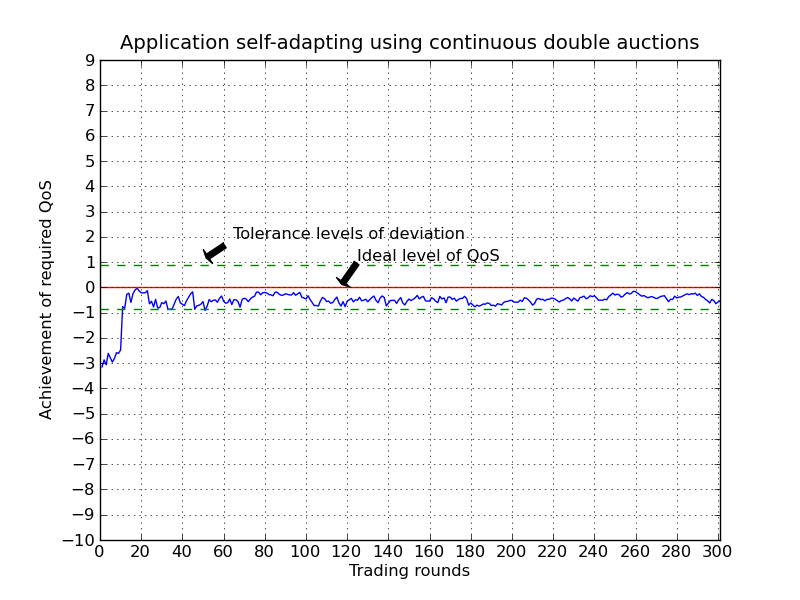
\includegraphics[width=3.8in]{graphs/Single_App_Self_Adaptation_Across_Rounds_With_QA_Change.png}
    \caption{The application quickly (within 10 trading rounds) achieves the utility associated with its desired QoS. Once it reaches the tolerance zone, it continually makes small adjustments to reach the ideal utility level. }
    \label{goodness}
\end{figure}	 
\subsubsection{Aggregate Perspective}
\textbf{Performance}:\\
We focus on the performance of the market as a whole in enabling applications to self-adapt. The market's performance is measured in terms of number of applications successfully able to achieve their target QoS. As a baseline, we first implement the Zero-Intelligence mechanism, as this represents the lower limit of the effectiveness of the CDA mechanism. The Zero-Intelligence scheme consists of agents randomly making bids and asks, with no history or learning or feedback(see figure \ref{pure_random_strategy}). As expected, it performs quite poorly, with only 10-20\% of applications managing to acquire the required QoS. Our mechanism achieves a much higher level of applications, able to attain their desired level of QoS(see figure \ref{marketperformance}). Adaptation using our mechanism allows 60-70\% of the applications in the market to adapt. Note, that this figure only indicates applications that have their QoS within the tolerance zone. There are many applications that have overshot their QoS requirements, but are unable to find sellers of services with lower QoS values. Depending on the distribution of QoS values amongst the sellers, this could represent skewedness in the market supply.\\
\textbf{Scalability Evaluation}:\\    
%ADD TEXT HERE THAT DISCUSSES ALL THE AXES AND GRAPHS SHOWING PERFORMANCE ALONG THOSE AXES
Another big advantage of our mechanism is its scalability. We measure the time taken for the market to perform matching with increasing number of concrete services available per abstract service in the application's workflow.  We see (in figure \ref{svc_scaling}), that the market mechanism is able to achieve an almost linear performance in time taken. Time is measured as the number of seconds taken for 300 rounds of trading.\\
\begin{figure}
    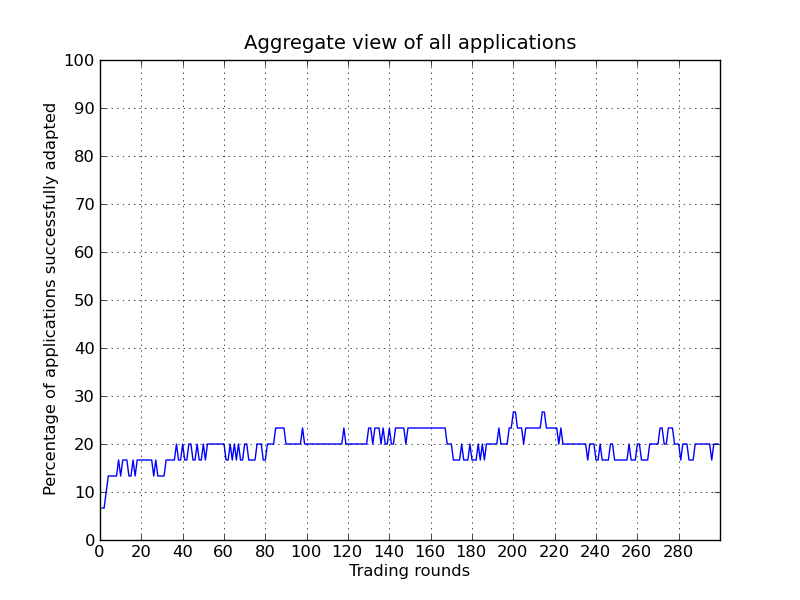
\includegraphics[width=3.8in]{graphs/efficiency-of-zi.png}
    \caption{Efficiency of using Zero-Intelligence. Unsurprisingly, applications using Zero-Intelligence are unable to satisfy their QoS requirements. On an average, only about 20\% of the applications in the market reach their desired QoS, which is clearly unsatisfactory.}
    \label{pure_random_strategy}
\end{figure}

\begin{figure}
	  %\\ \hline
	 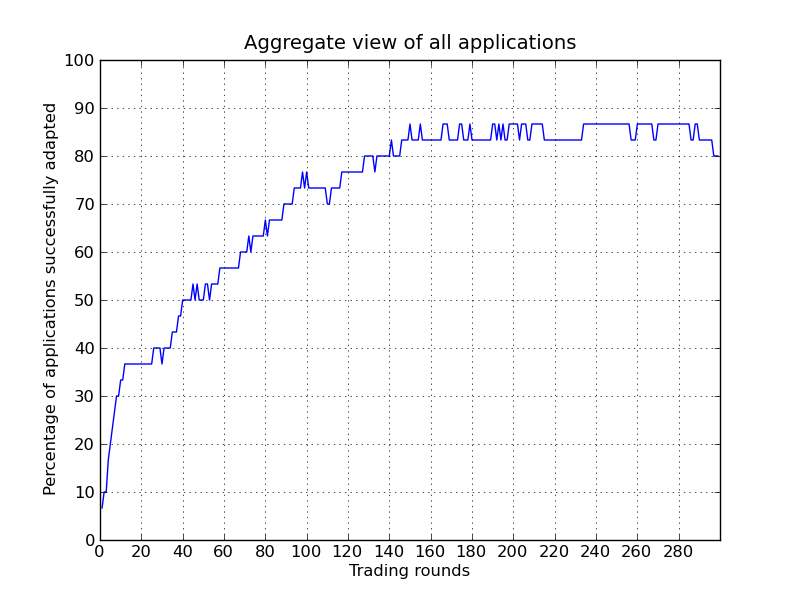
\includegraphics[width=3.8in]{graphs/probabilistic-change-to-qa.png}
	 \caption{We see that with adaptive bids, the number of applications that are able to adapt rise to about 85\% of the total market. This is a huge improvement with a very small improvement in the intelligence of the agents.}
	 \label{marketperformance}
       \end{figure} 
\begin{figure}
    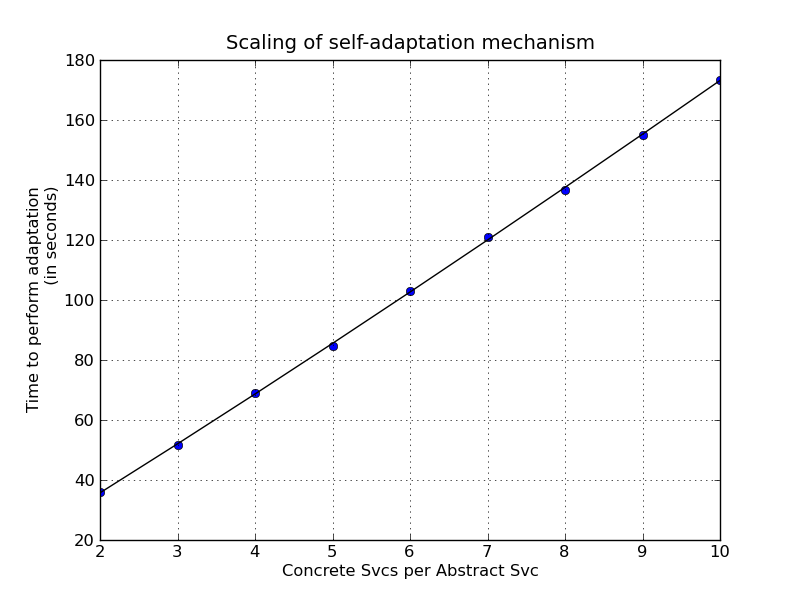
\includegraphics[width=3.8in]{graphs/Scaling-Num-ConcSvc-Per-Abstract-Svc.png}
    \caption{As the number of concrete services available per abstract service increases, the time taken to perform an auction also increases. However, the time taken increases linearly with the increase in concrete services. Each data point is the average of a 100 simulations each.}
    \label{svc_scaling}
\end{figure}

The number of QoS attributes per abstract service also affects the time taken by the market mechanism. 
% In figure \ref{qos_scaling}, we see that the time taken as the number of QoS attributes increase, is polynomial. 
Figure \ref{time_surface} shows the effect of increasing both, concrete services as well as QoS attributes, at the same time. We see that the surface is smooth and possess no peaks or troughs, thus indicating the consistent performance of the mechanism over a large input space. 
% \begin{figure}
%     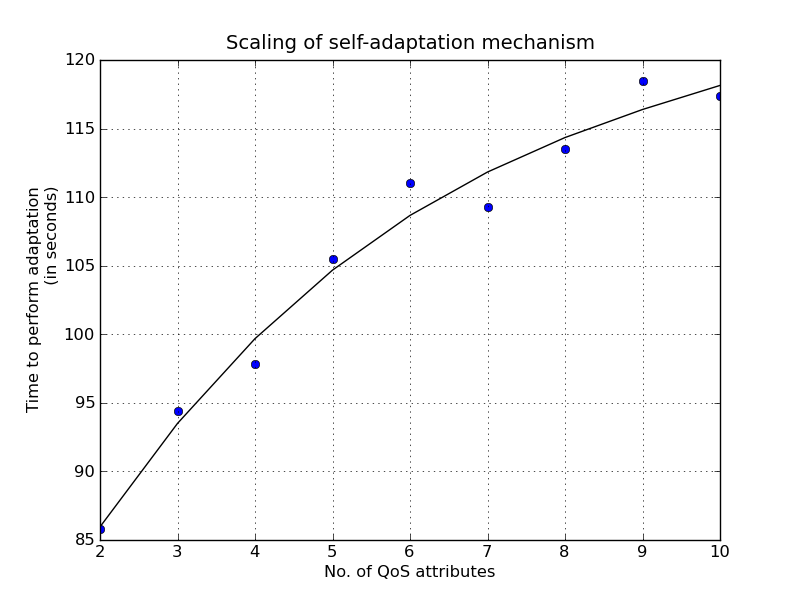
\includegraphics[width=3.8in]{graphs/Scaling_NumQA_Per_Svc.png}
%     \caption{Scaling of QoS attributes per Abstract Service}
%     \label{qos_scaling}
% \end{figure}

\begin{figure}
    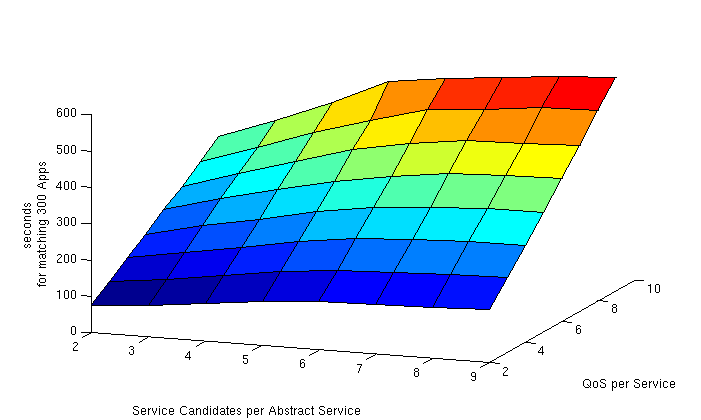
\includegraphics[scale=0.53]{graphs/Qa-vs-SvcCandidate-Time-Growth.png}
    \caption{The number of QoS attributes considered, also increases the time taken for adaptation. Increasing both the number of concrete services as well as QoS attributes reveals a smoothly increasing surface, without any sudden increase in time taken. The slope is steeper on the QoS axis, indicating that the adaptation is more sensitive to increase in QoS attributes, than to increase in choice of concrete services.}
     \label{time_surface}
\end{figure}

\textbf{Market Conditions}:\\
Investigating the effect of market conditions on the self-adaptive mechanism is slightly tricky. Conditions like paucity of supply, merely has the effect of less applications being able to satisfy their QoS requirements. The other conditions that we investigate are shown in Table \ref{MarketConditions}. As can be seen from the table, the changing of QoS attribute demand and/or supply, from a uniform distribution to a skewed (bimodal) distribution does not seem to adversely affect the performance, at the aggregate level. More investigation, however, is required to establish the limits at which the aggregate performance starts to degrade noticeably.
\begin{center}
\begin{table*}[ht]
 \begin{tabular}{| c | l | l |}
 \hline
 & \small Uniform Distribution of QoS in Sellers & \small Skewed Distribution of QoS in Sellers\\ \hline
 \small Uniform Dist of QoS in Buyers & 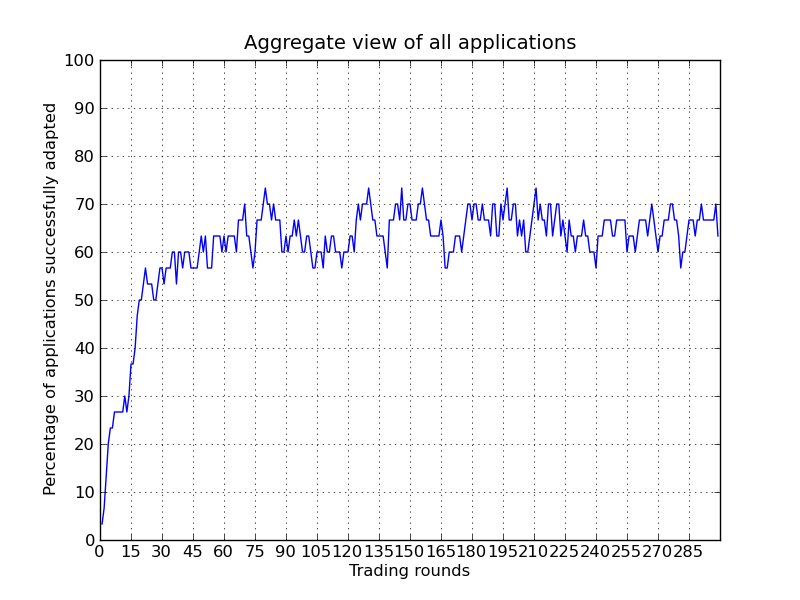
\includegraphics[scale=0.34] {graphs/uniform-seller-uniform-buyer.png} & 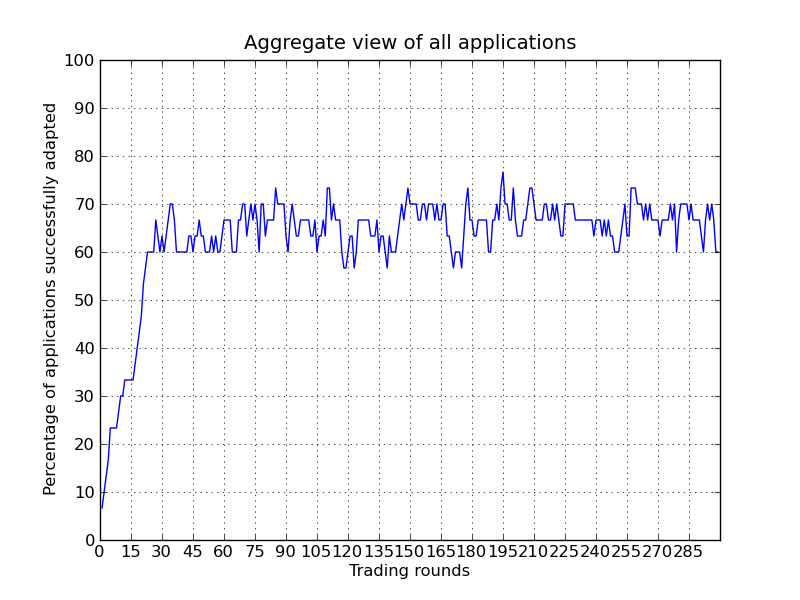
\includegraphics[scale=0.34] {graphs/uniform-seller-skewed-buyer.png}\\ \hline
 \small Skewed Dist of QoS in Buyers & 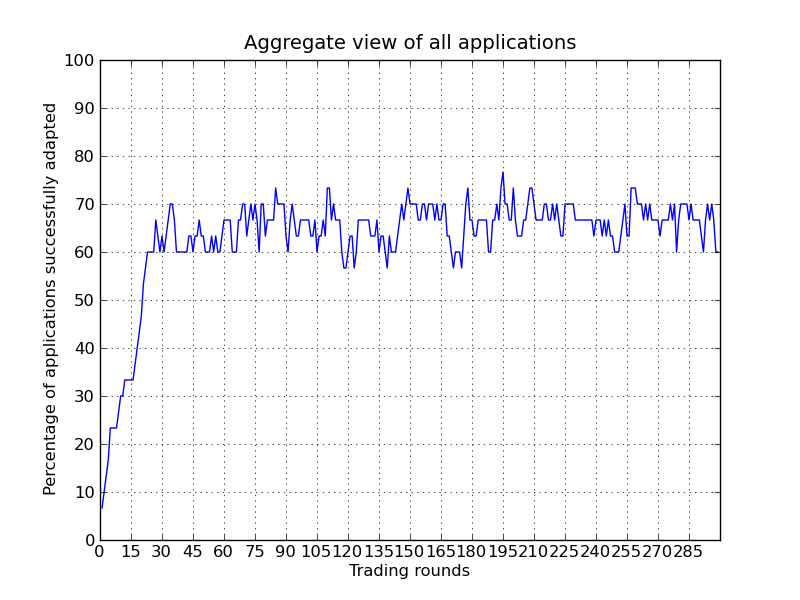
\includegraphics[scale=0.34] {graphs/uniform-seller-skewed-buyer.png} & 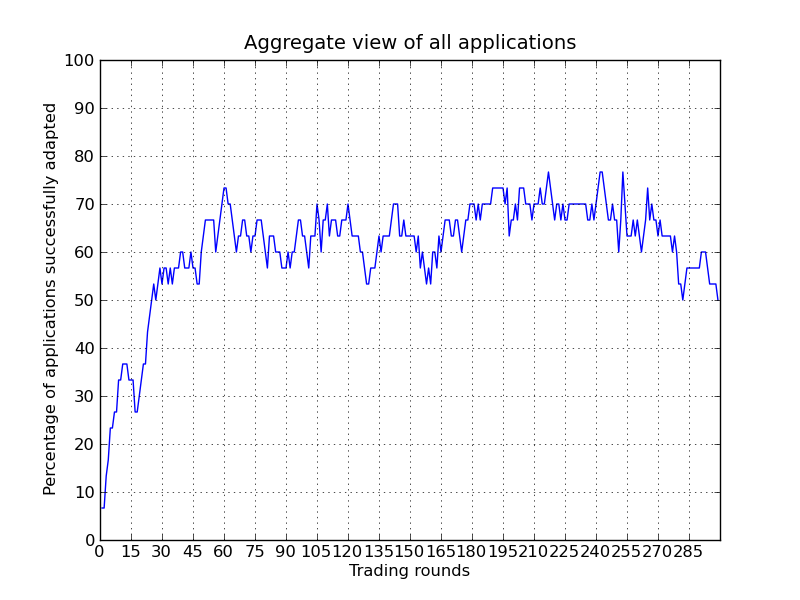
\includegraphics[scale=0.34] {graphs/skewed-seller-skewed-buyer.png} \\ \hline 
 \end{tabular}
 \caption[MarketConditions]{Depending on the kind of market conditions prevalent, applications find it easier/difficult to reach their target QoS levels. Predictably, we observe more fluctuation in the case of skewed supply and demand of QoS. Importantly though, in all four conditions, the macro behaviour of the system remains the same.} 
 \label{MarketConditions}
 \end{table*}
\end{center}
\textbf{Periodicity of Change}:\\
 In figures \ref{QoS_Change1} and \ref{QoS_Change2}, we compare the differences in the aggregate behaviour of all applications, when the periodicity of change of QoS is varied. In the first instance, we model all applications having independent probabilities of changing their target QoS attributes, over time. This means, any application could change its target QoS, at any point in time. In the second instance, we simulate an external event causing the applications to change their target QoS, every 25 rounds of trading.
       \begin{figure}
	 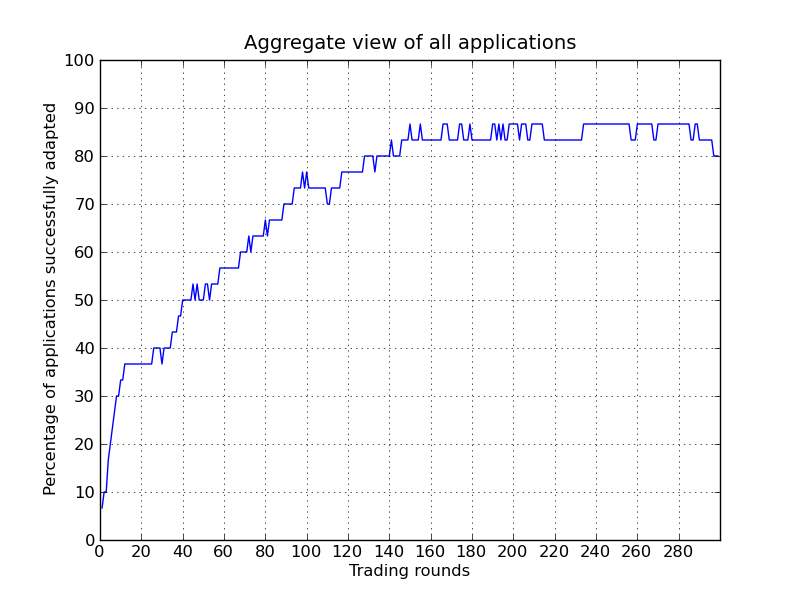
\includegraphics[width=3.8in]{graphs/probabilistic-change-to-qa.png}
	 \caption{Each application that succeeds in reaching its target, changes its target QoS with a small probability. We see that in the aggregate, there's not much change in the percentage of applications being able to self-adapt.}
	 \label{QoS_Change1}
       \end{figure}
	 \begin{figure}
	 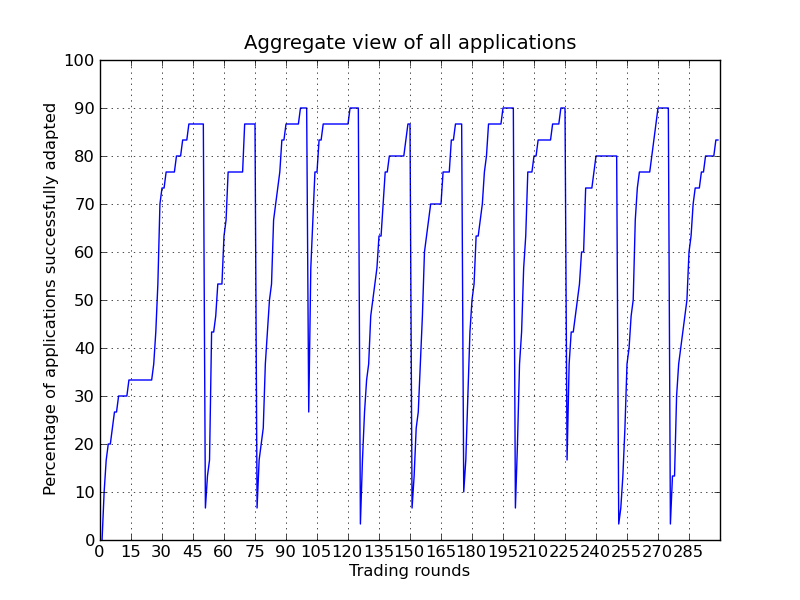
\includegraphics[width=3.8in]{graphs/periodic-change-to-qa.png}
	  \caption{Instead of a successful application changing its QoS, every application changes its target QoS at the completion of 25 trading rounds. This makes the aggregate adaption easier to see, since the market as a whole experiences a change in demand, periodically} 
	 \label{QoS_Change2}
	 \end{figure} %\\ \hline
%      \end{tabular}
     	
%  \end{table}
As expected, the periodic external event causes the aggregate number of satisfied applications to drop precipitously. Interestingly, it also causes the mechanism to satisfy a much higher percentage of the total applications. This is an interesting event and needs more investigation.

\subsection{Scalability Results}
\paragraph{With regard to size of workflow}
\paragraph{Number of candidate services}
\paragraph{Number of QoS constraints}
\paragraph{Number of markets}

\subsection{Discussion}
%DISCUSS PROS-AND-CONS OF ADOPTED ARCHITECTURAL STYLE. 
\subsubsection{Strengths}
A big strength of our mechanism is the high scalability that it offers. As service-oriented applications mature and cloud offerings become more standardized, it is easy to envision applications being composed out of several third-party services. In such a scenario, a mechanism that scales up to accommodate many concrete services is essential. We see that our mechanism is easily able to scale up.\\
Since the decision-making over which concrete service to instantiate is done in a de-centralized manner, the individual agents can be simple and easy to implement. \\    
Our mechanism implements a continuous adaptation scheme, thus leaving the system administrator free to attend to more critical tasks.

\subsubsection{Threats to Validity}

The set of services used to model the supply (as seen in table \ref{choice-of-services}) is deliberately seeded with services that probably will not be able to transact (e.g. $S1_{3}, S1_{54}, S3_{3}, S4_{3}$, etc.). This is done with a view to evaluating the mechanism's performance in an extreme situation. Services that advertise an availability of 79\% ($S1_{3}$) would never be acceptable.  In real life, these services would be competed out of the market, with most services differing in their QoS offerings by a marginal amount (or the price would be appropriately low, for low QoS). With a more typical scenario, our mechanim's performance would be much better, since the number of applications that're able to successfully achieve their QoS would be higher than figure \ref{marketperformance}. Since the self-adaptive mechanism merely attempts to satisfy the application's QoS targets, it does not try to achieve  optimal set of concrete services, even if available. This is a tradeoff that occurs between simplicity and robustness on one hand, and optimality on the other.\\

The market mechanism does not achieve the optimum, neither from the individual perspective nor from the aggregate perspective. Given the bounded rationality of our agents, we aim only to achieve a satisficing result, that is, find a solution that satisfies the constraints. 
% All satisficing problems can be trivially reformulated into optimization problems, but satisficing solutions need not be optimal solutions and vice-versa.\\

\textbf{Lack of Trust}: In any market-oriented mechanism, there is the issue of trust between the buyer of a service and the seller of a service. How does the seller reliably ensure that the buyer does not make more calls to the web-service, than the number agreed upon? How is the provenance of calls established? How does the buyer ensure that the seller provides the QoS, that it has promised in the SLA? What legal/technical recourse does it have, in case of violation of contract? These are all issues that are still open research problems. \cite{Ramchurn2005Trust} provides a good overview of these problems in the specific case of multi-agent systems. However, a good amount of research needs to be done, before all issues are acceptably resolved to the satisfaction of both, buyer and seller.\\
%\textbf{QoS Monitoring by External Entities}: Monitoring of QoS by third-party engines solve some of the trust issues discussed above, but introduce new ones. 

\section{Related Work}
    
\subsection{Dynamic Composition of Web-services} \label{dynamic_wsc}
There has been a plethora of work on dynamic composition of web-services. Much early work has been done in AgFlow \cite{Zeng2001AgFlow} on Quality-Aware composition of web-services \cite{Benatallah2002Declarative} and \cite{Zeng2003Quality}. The authors propose a per-service-class optimisation as well as a global optimisation using integer programming.\\
\cite{Canfora2005approach} proposed a genetic algorithm based approach where the genome length is determined by the number of abstract services that require a choice to be made. Constraints on QoS form a part of the fitness function, as do cost and other QoS attributes. A big advantage of GA-based approach is that it is able to handle non-linear constraints, as opposed to integer programming. Also, it is scalable when the number of concrete services per abstract service increase.\\
\cite{Alrifai2010Selecting} propose an interesting mechanism for cutting through the search space of candidate web-services, by using skyline queries. Skyline queries identify \textit{non-dominated} web-services on at least one QoS criteria. A \textit{non-dominated} web-service means, a web-service that has at least one QoS dimension in which it is strictly better than any other web-service and at least equal on all other QoS dimensions. Determining skyline services for a particular abstract service, requires pairwise comparisons amongst the QoS vectors of all the concrete services. This process can be expensive if the number of candidate concrete services is large. Alrifai et al. consider the case where the process of selecting skyline services is done offline. This would lead to an inability to adjust to changing conditions of available services and their associated QoS values. 	
\cite{Zhang2010QoS-Based} propose an interesting method to achieve a good set of concrete services, using Ant Colony Optimization (ACO). ACO involves creating virtual ants that mimic the foraging behaviour of real ants. The search space of optimal concrete services is modelled as a graph, with sets of concrete services as vertices and edges being all the possible connections between different concrete service sets. The ants attempt to complete a traversal of the graph, dropping pheromones on the edge of each concrete service visited. The path through the graph that accumulates the most pheromones represents the near-optimal path of services to use.
Our approach differs from the above approaches in two respects:
 \begin{enumerate}
     \item Consideration of time as a factor: In practice, the optimal set of concrete services may not be available at the time instant that an application is searching. The set of service providers changes with time, as does the set of service consumers. This means that the optimal matching of service providers to consumers changes with time. The approaches above do not take this into account.
     \item Optimality not considered: Due to the infeasibility of computing the optimal set (being NP-hard), we concentrate on finding a good solution, rather than an optimal one. A good solution is one that does not violate any QoS constraints and meets the cost constraint within a certain margin.
 \end{enumerate}

\subsection{Self-Adaptation}
Applications that use dynamic service composition should be able to continuously monitor their current QoS levels and make adjustments when either the demand for QoS changes or the cost constraint changes. The application should thus be able to respond to both internal as well as external stimuli, to trigger a change in its constituent web-services. This change needs to be both timely, as well as correct, \textit{i.e.}, the new set of services should not violate any of the application's QoS constraints, and the change should happen as fast as possible.\\
Self-Adaptation in software systems is the achievement of a stable, desirable configuration, in the presence of varying stimuli. These stimuli may be environmental (in the form of workload, failure of external components, etc.) or internal (failure of internal components, changed target states, etc.). Given that the range of stimuli that affect a software system is wide, Self-Adaptation has come to mean an umbrella term that covers multiple aspects of how a system reacts\cite{Salehie2009Self-adaptive}:
	\begin{enumerate}
	   \item Self-Awareness
	\item Context-Awareness
	\item Self-Configuring
	\item Self-Optimizing
	\item Self-Healing
	\item Self-Protecting 
	\end{enumerate}
However, most approaches to self-adaptation follow a common pattern: Monitor -- Analyze -- Plan -- Execute, connected by a feedback loop. There are two approaches to self-adaptation: centralized and de-centralized.  
In a centralized self-adaptive system, the analysis and planning part are concentrated in one entity. This form of self-adaptation has the advantage of cohesiveness and low communication overhead as compared to a decentralized mechanism. The analysis and the plan can be communicated to the effectors, and feedback from obeying the plan is communicated back through the monitors (or sensors). Rainbow\cite{Cheng2006Architecture-based} and \textit{The Autonomic Manager}\cite{IBM2006Architectural} are classic examples of centralized self-adaptation.\\
Decentralized self-adaptation, on the other hand, distributes the analysis, planning or the feedback mechanism amongst different parts of the adapting system. This automatically implies a communication overhead, since all constituent parts must coordinate their actions. However, it also provides for robustness in the presence of node failure and scalability of application size. \cite{Cheng2009Softwarea} have advocated that the feedback loop, which is a critical part of the adaptation, be elevated to a first-class entity in terms of modelling, design and implementation. Although, this would allow for reasoning about properties of the adaptation, there are no systems that we currently know of, that provide an explicit focus on the feedback loop. Most decentralized self-adaptation systems are typically realised as a multi-agent systems wherein the agents are autonomous in their environments and implement strategies that collectively move the entire system into a desirable state. \cite{Cheng2005Making} have advocated separating the functional part of the system from the adaptive part, thus allowing for independent evolution of both. \cite{Baresi2008Towards} describes such a system, where adaptation is considered as a cross-cutting concern, and not a fundamental part of system computation. Baresi et al. use aspect-oriented programming to implement the Monitor and Execute part of the MAPE loop. They implement distributed analysis and planning by dividing the self-adaptive system into \textit{supervised elements}, that perform the business logic of the application and \textit{supervisors} that oversee how the supervised components behave and plan for adaptation. Aspect-probes form the sensors and actuators that link the supervised elements to the supervisors. \\
\cite{Di2005Self-organization} describe another interesting approach to decentralized self-adaptation, through self-organization. DiMarzo et al. take a bio-inspired approach and use principles of holons (and holarchy) and stigmergy to get agents in a manufacturing department to perform coordination and control. A holon is defined by \cite{Koestler1990Ghost} to be both a part and a whole. Therefore, an agent is both autonomous as well as a part of a hierarchy, which influences it. The essential idea in their work is that with such structures, order emerges from disorder, as simple interactions build on each other, to produce progressively complex behaviour.\\
\cite{Weyns2010decentralized} study a decentralized self-healing system and a QoS-driven self-optimized deployment framework. Weyns et al.'s approach is the nearest to ours. They suggest multiple decentralized models which feed into decentralized algorithms, which are in turn analyzed by decentralized analyzers. These analyzers then individually direct local effectors to make changes to the host system.\\
These approaches, while interesting, have not explicitly considered scale of adaptation. Any approach that attempts self-adaptation on the cloud, must concern itself with scaling up to hundreds and possibly even thousands of entities. Another issue that needs to be considered, is the effect of other self-adapting systems operating in the same environment. 
 

\section{Conclusion and Future Work}
Cloud-based service-oriented applications have the potential to self-adapt their QoS, depending on demand. Using a market-based mechanism maps nicely to the real-world situation of unpredictable change of QoS requirements, costs involved in adaptation and adaptation by competing applications. As the number of possible concrete services increase, the scalability of the self-adaptive mechanism becomes important. We see that the market-based mechanism consists of simple agents, is able to adapt well and yet scales linearly to the number of concrete services. We also see that it is robust in the presence of differences in demand and supply of QoS. Applications implemented as an ASN can thus scale and adapt to the changing business requirements of QoS.\\
We have not modelled complex seller-side behaviour. Specifically, actions like deliberate violation of QoS to free up resources for making Asks with higher prices or mis-reporting of QoS available. Mechanisms like penalties and reputation management can be used to prevent seller agents from behaving dishonestly. Also, we have not modelled adaptation on the part of the market. Sellers that lie about their QoS or, are generally unattractive for transactions may lower the reputation of the marketplace. Hence, the market could take steps to ensure that it is populated, only with sellers that are likely to be sold. In future work, we aim to systematically add these adaptations to observe their effect on the collective economy. Also, future work involves experimenting with more decentralized market mechanisms such as posted-offer markets.\\
  
%  DISCUSS CLOUD-SIM IMPLEMENTATION\\
  

% Agile Service Networks embody the kind of structure, that this mechanism would be applicable in. Agile Service Networks are formed when organizations, outsource a part of their function to other organizations. These organizations may, in turn, outsource a part of their function to yet other organizations. Thus, an application or a business process being instantiated by one organization, uses the services of many organizations. This has several benefits in terms of efficiency, agility in response to business fluctuations etc.







    



\bibliographystyle{IEEEtran}
%\bibliography{/home/pg/vxn851/work/bibtex/viveknallur}
 \bibliography{viveknallur}

\begin{IEEEbiographynophoto}{Vivek Nallur}
Vivek did his undergraduate degree in business management and economics  from the University of Delhi. He, then went on to do a postgraduate diploma in advanced software technology and subsequently a Masters in Software Engineering, at Carnegie Mellon University, Pittsburgh. After working for six years in the industry, he is currently pursuing his PhD at the University of Birmingham, UK. His research interests are complex systems, decentralized self-adaptation and communication in multi-agent systems.
\end{IEEEbiographynophoto}

\begin{IEEEbiographynophoto}{Rami Bahsoon}
Dr. Rami Bahsoon is a Lecturer in Software Engineering at the School of Computer Science, the University of Birmingham, United Kingdom. He did his PhD from University College London (UCL), on evaluating software architectures for stability using real options theory. His research interests include Cloud Architectures, Security Software Engineering, Relating software requirements (non-functional requirements) to software architectures, testing and regression testing, software maintenance and evolution, software metrics, empirical evaluation, and economics-driven software engineering research.  
\end{IEEEbiographynophoto}

\end{document}